\section{Case 2}
For case 2 the linear multiple measurement vector model
\begin{align*}
\mathbf{Y} = \mathbf{AX},
\end{align*}
with $\mathbf{Y} \in \mathbb{R}^{m \times L}$ being a known measurement matrix, $\mathbf{A} \in \mathbb{R}^{m \times n}$ a known mixing matrix and $\mathbf{X} \in \mathbb{R}^{n \times L}$ being the source matrix we wish to recover in this case.
\\
The known matrices $\mathbf{Y}$ and $\mathbf{A}$ has been generated from a \texttt{sklearn}-package in Python. The commando used from this package is the \texttt{make\_sparse\_coded\_signal} with the inputs \texttt{(n\_samples = L, n\_components = n, n\_features = m, n\_nonzero\_coefs = k)}. The function generate a signal as a sparse combination of dictionary elements.
\\
The source matrix wish recovered $\mathbf{X}$ is also generated from this function and will be used to be compared with the recovered/estimated source matrix $\\hat{\mathbf{X}}$. $\hat{\mathbf{X}}$ will be recovered with the M-SBL Algorithm with the following variables: 
\begin{itemize}
\item $m = 10$ (number of sensors)
\item $n = 15$ (number of sources)
\item $L = 20$ (number of samples)
\item No segmentations -- $\mathbf{Y} = \mathbf{AX}$
\item Iterations = 1000
\item $k = 2$ is active sources (row-wise)($k$ is the non-zeros rows.)   
\end{itemize}
For the comparison we start with visualising the second row of $\mathbf{X}$ and $\hat{\mathbf{X}}$ which is one source ($n=1$) with $L = 20$ samples and the second column of $\mathbf{X}$ and $\hat{\mathbf{X}}$ which one sample $L=1$ with $n = 15$ sources.
\begin{figure}[H]
\centering
\begin{subfigure}{0.49\textwidth}
\centering
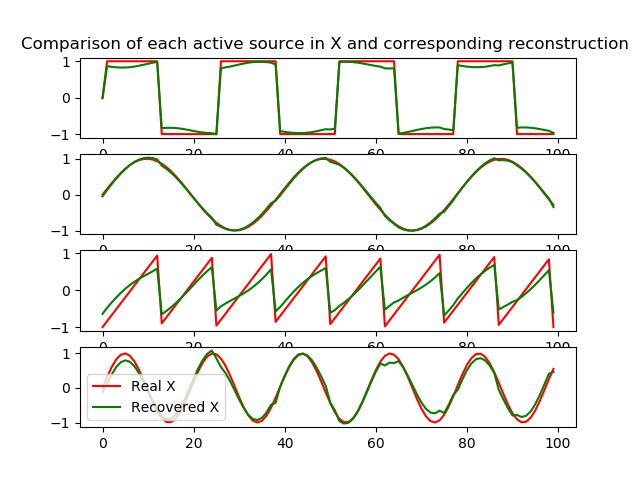
\includegraphics[width=\textwidth]{figures/cases/case2_1.png}
\caption{}
\label{fig:case2_1}
\end{subfigure}
\begin{subfigure}{0.49\textwidth}
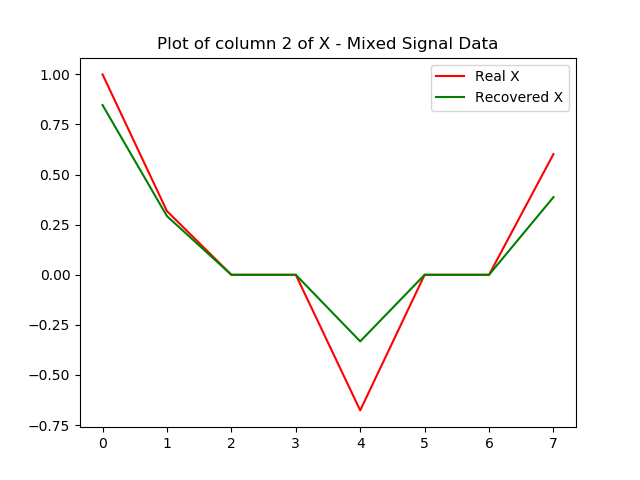
\includegraphics[width=\textwidth]{figures/cases/case2_2.png}
\caption{}
\label{fig:case2_2}
\end{subfigure}
\caption{\textbf{(a)} The comparison of one source of all the samples of the real $\mathbf{X}$ and the recovered $\hat{\mathbf{X}}$. \textbf{(b)} The comparison of one samples for all sources of the real $\mathbf{X}$ and the recovered $\hat{\mathbf{X}}$.}
\end{figure}
\noindent
We have found the error between all the elements of the known/real $\mathbf{X}$ and the recovered/estimated $\hat{\mathbf{X}}$ by using the mean square error (MSE):
\begin{align*}
\text{MSE} = \frac{1}{L} \sum_{i=1}^L (\mathbf{X} - \hat{\mathbf{X}}_i)^2
\end{align*}
The MSE of case 1 was found to be $0.037$ when rounded to the nearest three decimal.
\\ \\
As this case only have two active sources we provided the second plot.
\begin{figure}[H]
\centering
\begin{subfigure}{0.49\textwidth}
\centering
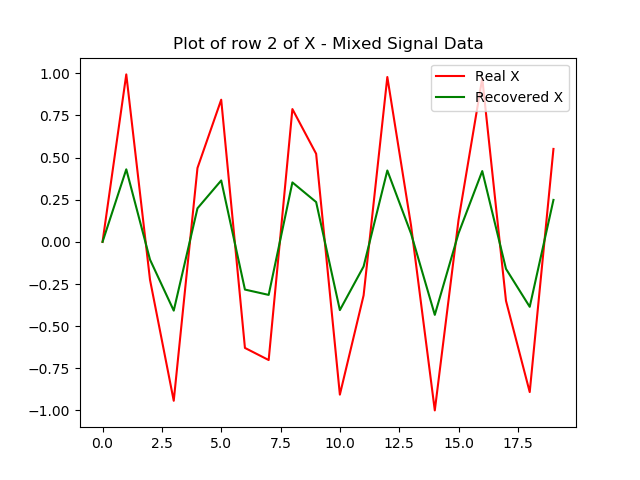
\includegraphics[width=\textwidth]{figures/cases/case2_3.png}
\caption{}
\label{fig:case2_3}
\end{subfigure}
\begin{subfigure}{0.49\textwidth}
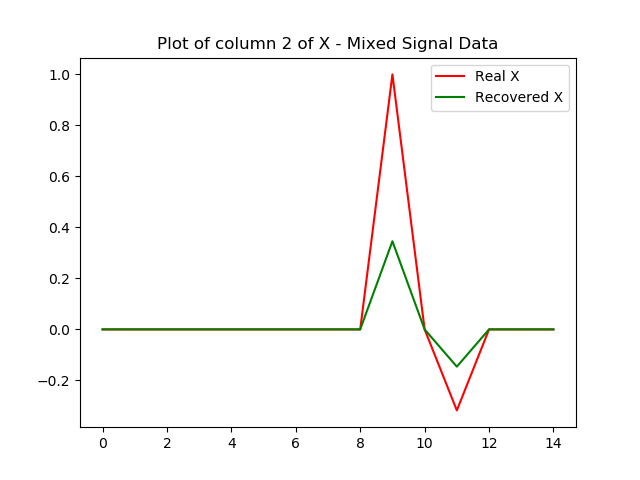
\includegraphics[width=\textwidth]{figures/cases/case2_4.png}
\caption{}
\label{fig:case2_4}
\end{subfigure}
\caption{\textbf{(a)} The comparison of one source of all the samples of the real $\mathbf{X}$ and the recovered $\hat{\mathbf{X}}$. \textbf{(b)} The comparison of one samples for all sources of the real $\mathbf{X}$ and the recovered $\hat{\mathbf{X}}$.}
\end{figure}
\noindent